\section{Conclusioni}
In questa sezione sono analizzate le performance dell'algoritmo \texttt{HeldKarp} e viene effettuato un confronto delle performance tra \texttt{TriangularTSP} e \texttt{CheapestInsertion}.

\subsection{HeldKarp}
%TODO

\subsection{CheapestInsertion e TriangularTSP}
Entrambi gli algoritmi sono una 2-approssimazione per TSP, ma riportano risultati differenti: \texttt{CheapestInsertion} richiede più tempo per essere eseguito rispetto a \texttt{TriangularTSP}, ma ottiene un errore relativo minore.\acapo

Per capire dunque quale dei due algoritmi sia più efficiente ed efficacie, è possibile osservare gli istogrammi a Figura~\ref{confronto} che mostra prima la differenza del tempo di esecuzione dei due algoritmi su scala logaritmica per i vari grafi, poi il tempo di esecuzione su una scala normale ed infine il rispettivo errore relativo. Confrontando il primo e terzo istogramma è possibile vedere come per un aggiunta di tempo di compilazione relativamente basso si ottiene un notevole miglioramento per l'errore relativo, infatti \texttt{TriangularTSP} raggiunge in media un errore relativo più alto ($\sim$32\%) rispetto a \texttt{CheapestInsertion} ($\sim$16\%). Se si osserva il secondo istogramma si può vedere come con grafi di taglia maggiore il tempo di esecuzione per \texttt{CheapestInsertion} aumenti esponenzialmente rispetto a \texttt{TriangularTSP}, basti osservare il tempo di esecuzione per i grafi \textit{d449} e \textit{dsj1000}.\acapo

Dunque per grafi di grande taglia è consigliabile utilizzare \texttt{TriangularTSP}, altrimenti \texttt{CheapestInsertion}.

\begin{figure}
	\centering
	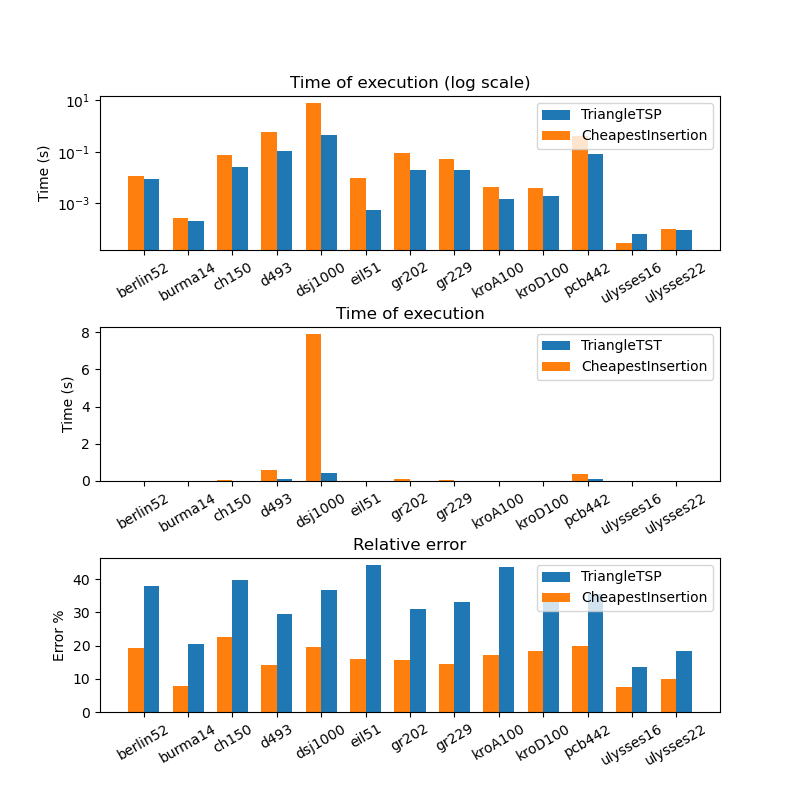
\includegraphics[width=\textwidth]{confronto}
	\caption{Confronto tra \texttt{CheapestInsertion} e \texttt{TriangularTSP}}
	\label{confronto}
\end{figure}
